% GENERATED by scripts/paper_figures.py from results/ -- do not edit
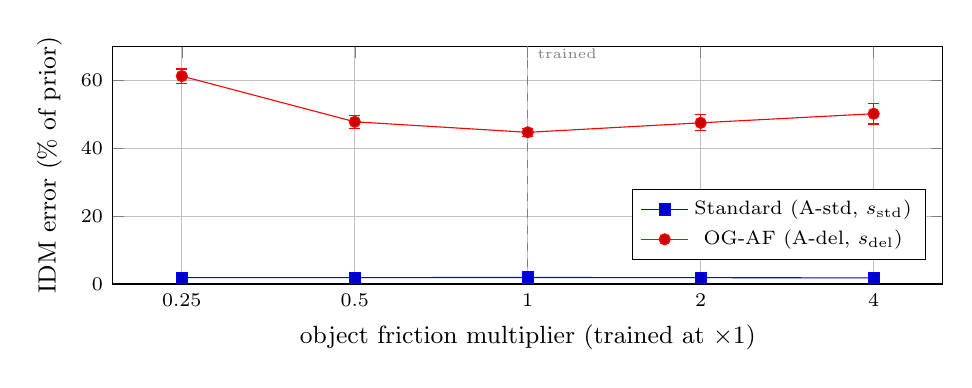
\begin{tikzpicture}\begin{axis}[width=\linewidth, height=4.6cm, xmode=log, log basis x=2,
  xlabel={object friction multiplier (trained at $\times1$)}, ylabel={IDM error (\% of prior)},
  xtick={0.25,0.5,1,2,4}, xticklabels={0.25,0.5,1,2,4}, ymin=0, ymax=70, grid=major,
  legend style={font=\scriptsize, at={(0.98,0.10)}, anchor=south east}, tick label style={font=\scriptsize},
  label style={font=\small}]
\draw[gray, dashed] (axis cs:1,0) -- (axis cs:1,70) node[pos=0.97, right, font=\tiny] {trained};
\addplot+[blue, mark=square*, error bars/.cd, y dir=both, y explicit] coordinates {(0.25,1.89541) +- (0,0.0934484) (0.5,1.89706) +- (0,0.0954691) (1,1.92642) +- (0,0.0554075) (2,1.88275) +- (0,0.119297) (4,1.80327) +- (0,0.126877)};
\addlegendentry{Standard (A-std, $s_\mathrm{std}$)}
\addplot+[red, mark=*, error bars/.cd, y dir=both, y explicit] coordinates {(0.25,61.2471) +- (0,2.07702) (0.5,47.7875) +- (0,1.92464) (1,44.6862) +- (0,1.15089) (2,47.4878) +- (0,2.33843) (4,50.1627) +- (0,3.02961)};
\addlegendentry{OG-AF (A-del, $s_\mathrm{del}$)}
\end{axis}\end{tikzpicture}
